%
% General structure for the revdetua class:
%
\documentclass[longpaper, english, final, times]{revdetua}
%
% Valid options are:
%
%   longpaper --------- \part and \tableofcontents defined
%   shortpaper -------- \part and \tableofcontents not defined (default)
%
%   english ----------- main language is English (default)
%   portugues --------- main language is Portuguese
%
%   draft ------------- draft version
%   final ------------- final version (default)
%
%   times ------------- use times (postscript) fonts for text
%
%   mirror ------------ prints a mirror image of the paper (with dvips)
%
%   visiblelabels ----- \SL, \SN, \SP, \EL, \EN, etc. defined
%   invisiblelabels --- \SL, \SN, \SP, \EL, \EN, etc. not defined (default)
%
% Note: the final version should use the times fonts
% Note: the really final version should also use the mirror option
%

\usepackage{amsmath, amsfonts, amssymb}
\usepackage{enumitem}
\usepackage{booktabs} % To thicken table lines
%\usepackage{longtable}
\usepackage{arydshln}
\usepackage{graphicx}
\usepackage{forest}


%% ALGORITHM 1 PROCEEDURES-----------------------------------------
%\usepackage{algorithm}
%%\usepackage[algo2e]{algorithm2e} 
%\usepackage{arevmath}     % For math symbols
%\usepackage[noend]{algpseudocode}

%% ALGORITHM 2 FUNCTIONS-----------------------------------------
\usepackage{xcolor}
\usepackage[linesnumbered,ruled,vlined]{algorithm2e}
% set comment color to blue
\newcommand\mycommfont[1]{\footnotesize\ttfamily\textcolor{blue}{#1}}
\SetCommentSty{mycommfont}
\begin{document}
	
	%\Header{Volume}{Number}{Month}{Year}{InitialPage}
	% Note: the month must be in Portuguese
	
	\title{The Warehouse Location Problem}
	\author{ABLORDEPPEY Prosper (106382)} % or \author{... \and ...}
	\maketitle
	
	\begin{abstract}% Note: in English
%		know kcenter problem is, given n cities with specified distances, one wants to build k warehouses in different cities and minimize the maximum distance of any city to a warehouse.
%		
%		In this problem, the number of warehouses is fixed to k, and the goal is minimizing the maximum distance between any city to it's the nearest warehouse.
		Given $n$ cities with specified distances, one wants to build $k$ warehouses in different cities and \textit{minimize} the maximum distance of any city to a warehouse. This presentation seeks to solve the metric facility location problem by designing, testing and analyzing results from three (3) different algorithms based on an exhaustive search, a greedy heuristic, and a randomized implementation.\\
		
		In graph theory this problem is referred to as $k-center$ problem which is NP-Hard, formulated as; 
		given a weighted complete undirected graph $\mathcal{G(V, E, W)}$, with $\mathcal{V}$ the set of vertices, $\mathcal{E}$ the set of edges and $\mathcal{W}$ is the set of weights/distances (euclidean) between any two vertices of the graph, we aim to find a set of $k \leq m$ vertices for which the largest distance of any other vertex to its closest vertex in the k-set is minimum.\\
		
		The project further compares the solutions generated by the different approaches for some example problem instances. Afterwards, we carry out systematic computational experiments and analyze the computational complexity of the developed algorithms for prime numbers $k \in \{2,3,5,7,\dots\}$.
	\end{abstract}
%
%	\section{dummyref}
%		\cite{adjacencymatrixdefinition}
%		\cite{GONZALEZ1985293}
%		\cite{black2012greedy}
%		\cite{erdos1959random}
%		\cite{kcenterProblem}
%		\cite{hui2010study}
%		\cite{powerset_generation}
%		\cite{horvitz1952generalization}
%	
%	\begin{resumo}% Note: in Portuguese
%		...
%	\end{resumo}
	
	\begin{keywords}% Note: in English (optional)
		\begin{itemize}
			\item $n=\mathcal{|V|}$ - the number of vertices of graph $\mathcal{G}$.
			\item $m=\mathcal{|E|}$ - the number of edges of graph $\mathcal{G}$.
			\item $(u,v) \in \mathcal{E}$ - is an edge of $\mathcal{G}$.
			\item $w((u,v)) \in \mathcal{W}$ - is the euclidean distance between the edge connecting $u, v \in \mathcal{V}$ for $(u,v)\in \mathcal{E}$. Thus $\mathcal{W}:\mathcal{E}\rightarrow \mathbb{Z^+}$
			\item $\mathcal{V^{*}}$ - a subset of $\mathcal{V}$ of size $\left(k\leq n\right)$ where the warehouses should be located/built, in order to minimize the maximum distance of the cities from a warehouse. More formally, $\mathcal{V^{*}}\subseteq \mathcal{V} \ni \sup_{v\in \mathcal{V}}w_{\mathcal{G}(v, \mathcal{V^{*}})}$ is minimized \cite{kcenterProblem}.
			\item $Adj_\mathcal{G}$ - the adjacency matrix of graph $\mathcal{G}$, is a two dimensional (2D) matrix of weights/euclidean distances connecting pair of vertices in the network. \cite{adjacencymatrixdefinition}.
			\item counter - the number of operations carried out for each $k$.
		\end{itemize}
	\end{keywords}
	
%	\begin{palavraschave}% Note: in Portuguese (optional)
%		...
%	\end{palavraschave}

	\section{Outline Of Implementation}
		The outline of this project is given as follows;
		\begin{enumerate}[label=(\arabic*)]
			\item[\ref{outline:project-structure}.] Project Directory Structure 
			\item[\ref{outline:exhaustive}.] Brute-Force or Exhaustive-Search
			\item[\ref{outline:greedy}.] Greedy-Heuristic
			\item[\ref{outline:randomized}.] Randomized Approach
			\item[\ref{outline:formal-analysis}.] Formal Analysis
			\item[\ref{outline:practical-analysis}.] Practical Analysis
			\item[\ref{outline:example-case}.] Example Case ($n=5$, $k\in [2,3]$)
		\end{enumerate}
	
	\section{\label{outline:project-structure} Project Directory Structure}
	
		The folder structure for this project is graphically given in Fig. (\ref{figure:projectDirectoryStructure}). 
		From the representation, the project has one (1) main directory and the \textit{Warehouse\_Location} python notebook file. Detailed description is presented below;
		\begin{figure}[!ht]
			\begin{center}
				\begin{forest}
					for tree={
						font=\ttfamily,
						grow'=0,
						child anchor=west,
						parent anchor=south,
						anchor=west,
						calign=first,
						edge path={
							\noexpand\path [draw, \forestoption{edge}]
							(!u.south west) +(7.5pt,0) |- node[fill,inner sep=1.25pt] {} (.child anchor)\forestoption{edge label};
						},
						before typesetting nodes={
							if n=1
							{insert before={[,phantom]}}
							{}
						},
						fit=band,
						before computing xy={l=15pt},
					}
					[Project
					[graphs
					[pickles
						[2\_nodes.gpickle]
						[3\_nodes.gpickle]
						[...]
						[19\_nodes.gpickle]
						[20\_nodes.gpickle]
					]
					[plot\_output
						[exhaustive\_n5\_k2.png]
						[exhaustive\_n5\_k3.png]
						[greedy\_n5\_k2.png]
						[greedy\_n5\_k3.png]
						[randomized\_n5\_k2.png]
						[randomized\_n5\_k3.png]
						[n5.png]
					]
					[executions
						[exhaustive.csv]
						[greedy.csv]
						[randomized.csv]
					]
					]
					[Warehouse\_Location.ipynb]
					]
				\end{forest}
			\end{center}
			\caption{Project Directory Structure}
			\label{figure:projectDirectoryStructure}
		\end{figure}
	
		\begin{itemize}
			\setlength\itemsep{1em}
			\item \textbf{graphs} \\
				This folder hosts two (2) sub-directories as detailed below; 
				\begin{enumerate}
					\item \emph{pickles} :- This directory holds all the graphs generated and saved in $gpickle$ format for the $networkx$ library. In total, eighteen (18) graphs were generated, with number of vertices ranging from $(2-20)$ as shown in the output of Fig (\ref{figure:projectDirectoryStructure}).
					\item \emph{plot\_output} :- This directory also holds the output of the graphs generated using each of the implemented algorithms for varying \emph{k-sets} considered. The output of Fig (\ref{figure:projectDirectoryStructure}) shows output of the search algorithms implemented using the graph with five (5) vertices.
					\item \emph{executions} :- The repository contains csv register of \textit{counter values}, \textit{output of optimal locations} and \textit{time} it took to find a solution for each \emph{k-set} considered for a given \textit{vertex}. As seen from the tree representation, there are only three (3) registers/files in this sub-folder.
				\end{enumerate}
			
			\item \textbf{Warehouse\_Location.ipynb} \\			
			This is the python notebook file generating the \textit{graphs} and \textit{plot\_output} files detailed above. \\
						
			All the implementations were done in Python. The packages used were; numpy, shutil, os, time,itertools, networkx and matplotlib. The functions for which these packages were used are detailed in the $warehouse_location.ipynb$ file.
			
			This file implements two (2) classes as detailed below; \\
			\begin{itemize}
				[topsep=1ex,itemsep=1ex,partopsep=1ex,parsep=1ex]
%				\setlength\itemsep{1em}
				\item \textbf{IOBASE Class} (Input/Output Operations) \\
					We employed six (6) functions to help with the implementation of this project. They are;
					\begin{enumerate}[label=\arabic*), topsep=0pt,itemsep=0ex,partopsep=1ex,parsep=1ex]
						\item CreateDirectory
						\begin{itemize}
							[topsep=0pt,itemsep=-1ex,partopsep=1ex,parsep=1ex]
							\item create directories to hold graphs and plots.
							\item deletes directories as requested.
						\end{itemize}
						\item GenerateNodeCoordinates
						\begin{itemize}
							[topsep=0pt,itemsep=-1ex,partopsep=1ex,parsep=1ex]
							\item After successful generation og \emph{Erdos Renyi Graphs}, for consistency with the preamble, this method generates integer valued coordinates to each vertex in the XOY plane between 1 and 1000.
						\end{itemize}
						\item ComputeEdgeDistances
						\begin{itemize}
							[topsep=0pt,itemsep=-1ex,partopsep=1ex,parsep=1ex]
							\item the euclidean distance between the source and sink of each edge of the graph is computed in this method. The Euclidean distance is expressed as;
							$$ w((u,v))=\sqrt{\sum_{i=1}^{2}(u_i-v_i)^{2}}$$
							\item for a cleaner representation, the computed distances were rounded to the nearest whole number.
						\end{itemize}
						\item GenerateGraphs
						\begin{itemize}
							[topsep=0pt,itemsep=0ex,partopsep=1ex,parsep=1ex]
							\item implements the generation of random \emph{Erdos Renyi Graph} for specified number of vertices.
							\item fetch integer valued coordinates (between 1-1000) for all vertices (from \emph{GenerateNodeCoordinates}) to update graph.
							\item fetch computed euclidean distances (from \emph{ComputeEdgeDistances}) for all edges to update the graph. 
							\item plot graphs after generation.
							\item save the graph to current graphs directory in $gpickle$ format.
						\end{itemize}
						\item LoadGraph
						\begin{itemize}
							[topsep=0pt,itemsep=-1ex,partopsep=1ex,parsep=1ex]
							\item load a graph from file.
							\item plot the graph if requested.
						\end{itemize}
						\item PlotGraph
						\begin{itemize}
							[topsep=0pt,itemsep=-1ex,partopsep=1ex,parsep=1ex]
							\item main implementation of graph plotting.
							\item weighted or not weighted.
							\item partial coloring of given vertices.
						\end{itemize}
					\end{enumerate}
				\item \textbf{WarehouseLocation Class} (main implementation) \\
					This is the main class that implements the search algorithms, namely; Exhaustive Search, Greedy and randomized Algorithms. A method for generating the prime numbers used for $k$ was also implemented. 
			\end{itemize}
		\end{itemize}
	
	 	
	\section{\label{outline:exhaustive} Exhaustive-Search Implementation}
		Exhaustive search means we try every possible solution to the problem and choose the best one that satisfies the objective. The main strength of the Exhaustive Search is that it is guaranteed to find the best optimal solution from all possible solutions, in this case, a \emph{k-set} subset of all cities which minimizes the largest distance of any other city to its closest city in the \emph{k-set} subset selected \cite{hui2010study}.\\
		
		The solution to this problem is a subset of the vertices set. So in this case, it means we figure out all \emph{k-set} subsets of the vertices set which are potential solutions to our problem. The \emph{k-set} subset which $minimizes$ the $largest$ distance of any other city to its $closest$ warehouse in the \emph{k-set}  is our optimal solution to the warehouse locations problem.\\
		
		The deficiency of this algorithm is that it takes a long time to complete execution for graphs with larger vertices and/or edges \cite{hui2010study}. \\
		
		The \textbf{Algorithm \ref{algorithm:potentialVStar}} is a helper function for the main implementation of the Exhaustive Search as presented in \textbf{Algorithm \ref{algorithm:exhaustiveSearch}}. In its implementation, the goal is to generate all non-empty, \emph{k-set} subsets of the given vertices set $\mathcal{V}$. We obtain such sets by considering the powerset $(\rho)$ of $\mathcal{V}$. The function returns a list of tuples, each comprising of a subset of length $k<|\mathcal{V}|$. Each of these subsets are potential solutions to be investigated in the main function as described in \textbf{Algorithm \ref{algorithm:exhaustiveSearch}}. \\
		
		\begin{algorithm}[!h]
			\caption{Generate Potential $\mathcal{V^{*}}$s}
			\label{algorithm:potentialVStar}
			\SetKwInput{KwInput}{Input}              % Set the Input
			\SetKwInput{KwOutput}{Output}              % set the Output
			\DontPrintSemicolon
			
			\KwInput{$\mathcal{V}$, $k$ \tcp*{$\mathcal{V}$:vertices set, $k$:\# locations}}
			\KwOutput{$p\_sets$ \tcp*{potential locations list}}
			
			% Set Function Names
			\SetKwFunction{FMain}{PotentialVStars}
			
			% Function Definition			
			\SetKwProg{Fn}{Function}{:}{\KwRet}
			\Fn{\FMain}{
				Set $p\_sets \gets$ [ ]  \;%
				Set $\rho \gets$ Powerset($\mathcal{V}$)  \tcp*{length $2^{|\mathcal{V}|}$}
				\ForEach{$subset \in \rho$}{%
					\tcp{non-empty subsets each of size $k$\
					}	
					\uIf{($subset\neq \emptyset$) or ($subset \neq \mathcal{V}$)}{
						\uIf{\emph{len($subset$)} $== k$}{
							$p\_sets\cdot$insert($subset$) \;	
						}
					}
				}
				\KwRet $p\_sets$\;
			}
		\end{algorithm}
		
		\begin{algorithm}[!h]
			\caption{Exhaustive Search}
			\label{algorithm:exhaustiveSearch}
			\SetKwInput{KwInput}{Input}                % Set the Input
			\SetKwInput{KwOutput}{Output}              % set the Output
			\DontPrintSemicolon
			\KwInput{$\mathcal{G(V,E, W)}$, $k$ \tcc*{G:graph, k:locations}}
			\KwOutput{$\mathcal{V^{*}}$ \tcp*{optimal k-set locations}}
			
			% Set Function Names
			\SetKwFunction{FMain}{ExhaustiveSearch}
			
			% Function Definition			
			\SetKwProg{Fn}{Function}{:}{\KwRet}
			\Fn{\FMain}{%
				\tcc{
					$\mathcal{V^{*}}$ - optimal warehouse locations.\;
					$p\_vstar$ - potential $\mathcal{V^{*}}$s.\;
					$p\_sets$ - set of $p\_vstar$.\;
					$ol\_max\_dist$ - list of $p\_vstar$ with largest distance from cities.
				}
				Set  $p\_sets \gets$ PotentialVStars($\mathcal{V}$, $k$)\;
				Set $pv\_max\_d \gets \{p: -\infty \ni \forall p \in p\_sets \}$\;
				\ForEach{$p\_vstar \in p\_sets$}{%
					$c\_dists \gets $ [ ] \tcp*{closest dist from $p\_vstar$}
					\ForEach{$vertex \in \mathcal{V}$}{
						\tcc{
							find closest distance from $p\_vstar$, for every city\;
							update $c\_dists$
						}						
						$d \gets \text{Adj}_\mathcal{G}[vertex]$ \tcp*{neighbour dists}
						$ds\_from\_pvstar \gets$ $d$ from $p\_vstar$\;
						$c\_dists \cdot$add$( \text{min}(ds\_from\_pvstar))$
					}
					$largest\_dist\gets $max($c\_dists$)\;
					\uIf{$largest\_dist > pv\_max\_d[p\_vstar]$}{
						$pv\_max\_d[p\_vstar]\gets largest\_dist$
					}
				$V\_star\gets$ min($pv\_max\_d$)
				}
				\KwRet $V\_star$\;
			}
		\end{algorithm}
		
		First, we get all the various subsets of $\mathcal{V}$ that have equal chance of being the optimal solution of interest ($\mathcal{V^{*}}$) using the $PotentialVStars$ function in \textbf{Algorithm \ref{algorithm:potentialVStar}}. We find the largest distance of the closest city/vertex in the graph to these potential optimal solutions. The optimal solution ($\mathcal{V^{*}}$) is the set corresponding to the minimum distance.\\
			
		For each of the element of the array or potential optimal location set, we then compute the largest distance of the closest city to vertices making up the set of the element. The minimum is then returned as the optimal location for the warehouses.
		
	\section{\label{outline:greedy} Greedy-Heuristics Implementation}
		A Greedy algorithm is any algorithm that follows the problem-solving heuristic of making a locally optimal choice at each stage \cite{black2012greedy}. In many problems, a greedy strategy does not produce an optimal solution, but a greedy heuristic can yield locally optimal solutions that approximate a globally optimal solution in a reasonable amount of time, where as an exhaustive search will look at all possible solutions and pick the most optimal one. Thus, the Greedy heuristics runs faster as compared to the Exhaustive search.\\
		
		A solution to this warehouse location problem, was given
		by \cite{GONZALEZ1985293} in 1985 using a greedy heuristics. In this algorithm, we build the set $\mathcal{V^{*}}$ by iteratively adding a vertex to which is farthest from the set of vertices we have already chosen. We keep doing this until
		we have chosen $k$ vertices as implemented in Algorithm (\ref{algorithm:GreedyAlgorithm}). The algorithm implements a random initialization of the first member of $\mathcal{V^{*}}$. This algorithm is a modified version of the vanilla randomized approach described under the Randomized implementation \ref{outline:randomized} (random sampling $k$ vertices from $\mathcal{V}$), constraint on the fact that, new vertices added to $\mathcal{V^{*}}$ are farthest away from members of $\mathcal{V^{*}}$. This thereby increases the chance of realizing if not the true warehouse locations set, but an estimate very close to the true set. This is further confirmed in the following sections.\\
		
		\begin{algorithm}
			\caption{Greedy Heuristics}
			\label{algorithm:GreedyAlgorithm}
			\SetKwInput{KwInput}{Input}                % Set the Input
			\SetKwInput{KwOutput}{Output}              % set the Output
			\DontPrintSemicolon
			
			\KwInput{$\mathcal{G(V,E,W)}$ \tcc*{G:graph, k:locations}}
			\KwOutput{$\mathcal{V^{*}}$ \tcp*{warehouse locations $\mathcal{V^{*}}\subseteq \mathcal{V}$}}
			
			% Set Function Names
			\SetKwFunction{FMain}{GREEDY}
			
			% Function Definition			
			\SetKwProg{Fn}{Function}{:}{\KwRet}
			\Fn{\FMain}{
				Set $\mathcal{V^{*}} \gets \emptyset$ \;%
				$\mathcal{V^{*}}\cdot $add(random($v \in \mathcal{V}$))\;
				\For{$iter$ \emph{in} \textit{range(k-1)}}{
					Set $max\_dist \gets -\infty$ \tcp*{maximum trick}%
					Set $max\_dist\_node \gets None$\;%
					\ForEach{$node \in \mathcal{V}$}{
						\ForEach{$sel\_node\in \mathcal{V^{*}}$}{
							\tcp{distance from adj. matrix}
							\textit{dist} $\gets$ Adj$_{\mathcal{G}}$[$node$][$sel\_node$]\;
							\If{$dist < max\_dist$}{
								$max\_dist\_node \gets node$
							}
						}
					}
					$\mathcal{V^{*}}\cdot $add($max\_dist\_node$)
				}
				\KwRet $\mathcal{V^{*}}$\;
			}
		\end{algorithm}
	
	
	\section{\label{outline:randomized} Randomized Implementation}
	
		The Randomized approach as described in \textbf{Algorithm \ref{algorithm:RandomizedAlgorithm}} provides a naive solution to the warehouse location problem. The algorithm selects $k$ random unique vertices one (1) at a time. In probability theory, this sampling technique is known as Sampling Without Replacement. As a result, the distances between vertices pair, which are of high essence to satisfying the objective function is disregarded. \\
		
		In order to improve the output/result of the randomized approach presented, we can decide to run the algorithm multiple times and report the location set which minimizes the largest distance of any other city as the optimal solution set. Another approach as presented in the Greedy Search implementation \ref{algorithm:GreedyAlgorithm} partially fulfills the objective function could be considered.
		
		\begin{algorithm}[h]
			\caption{Randomized Algorithm}
			\label{algorithm:RandomizedAlgorithm}
			\SetKwInput{KwInput}{Input}                % Set the Input
			\SetKwInput{KwOutput}{Output}              % set the Output
			\DontPrintSemicolon
			
			\KwInput{$\mathcal{G(V,E,W)}$, $k$ \tcc*{G:graph, k:locations}}
			\KwOutput{$\mathcal{V^{*}}$ \tcp*{optimal locations set estimate}
			}
			
			\SetKwRepeat{Do}{do}{while}
			
			% Set Function Names
			\SetKwFunction{FMain}{ProbabilisticRandomized}
			
			% Function Definition			
			\SetKwProg{Fn}{Function}{:}{\KwRet}
			\Fn{\FMain}{
				Set $\mathcal{V^{*}} \gets \emptyset$\;
				\For{$iter$ \emph{in} \textit{range(k)}}{
					\tcp{choose random vertex from $\mathcal{V}$}
					\emph{selected} $\gets$ rand($\mathcal{V}\backslash \mathcal{V^{*}}$)\;
					$\mathcal{V^{*}}\cdot$add(\emph{selected})
				}
				\KwRet $\mathcal{V^{*}}$\;
			}
		\end{algorithm}
		
	\section{\label{outline:formal-analysis} Formal Analysis}
		This section presents a formal analysis of the complexities and running times of the exhaustive-search algorithm described in \textbf{Algorithm \ref{algorithm:exhaustiveSearch}}, the greedy implementation in \textbf{Algorithm \ref{algorithm:GreedyAlgorithm}} and the randomized approach as described in \textbf{Algorithm \ref{algorithm:RandomizedAlgorithm}}.
		
		\subsection{Exhaustive Search}
			Considering a connected graph with $n$ vertices. Thus, $|\mathcal{V}|=n$. If $p\_sets$ is the set of all potential optimal location sets of $\mathcal{V^{*}}$. An expression for the cardinality of $p\_sets$ is given as
			$$|p\_sets|={n\choose{k}} = \frac{n!}{k!\cdot (n-k)!}$$. \\
			
			Given a set with $n$ elements, the total number of different subsets that can be obtained from the set is expressed as $|\rho|=2^n$\cite{powerset_generation}. From the implementation of the helper function as described in \textbf{Algorithm \ref{algorithm:potentialVStar}}, we generated the power-set of the vertices set ($\rho$) and filtered it to obtain our desired list of potential optimal location set. Since our interest is to obtain non-empty subsets of size $(k<|\mathcal{V}|)$, we eliminate the empty set $(\emptyset)$ and the set with the full vertices. This results in $(2^{n}-2)$ subsets returned by this function. The complexity of this algorithm runs in exponential time given as $C = \mathbf{\mathcal{O}(2^n)}$.\\
			
			The main implementation finds the largest distance of the closest city for each potential optimal location set and stores the result in an associative array. This is achieved by going over each of the $n$ vertices. The key with the smallest/minimum distance is our desired optimal location set for our warehouse location problem.\\
			
			Summing it all up, the Exhaustive Search implementation of the warehouse facility problem runs in complexity
			\begin{align*}
				C & = \mathcal{O}\left(2^n \cdot n\right) \\
				& = \mathbf{\mathcal{O}\left(2^{n}\right)}
			\end{align*}
			Exponential running time algorithms like this is one of the worse algorithms to have for larger graph inputs if we want to obtain result within the fastest time which is impossible but will guarantee optimal solution.
			
		\subsection{Greedy Search}
			As studied in the Randomized implementation, the probability of any of the members of $p\_sets$ being the optimal location set the becomes
			$$\mathcal{P}=\frac{1}{{n\choose k}}$$ The Greedy Heuristics improves this probability constraint on the basis that new vertices selected have their distances from the selected vertices largest compared to the other not selected vertices. This ensures an increased chance of obtaining the optimal warehouse location set as compared to the naive randomized implementation.\\
			
			According to \cite{kcenterProblem}, this algorithm runs in polynomial-time and provides a solution that is never worse than twice the optimal solution, which always work only if the distances between cities follow Triangular Inequality (the distance between two points is always smaller than the sum of distances through a third point. This condition is satisfied by the euclidean distance \cite{greenhoe2016properties}.\\
			
			The Greedy approach in \textbf{Algorithm (\ref{algorithm:GreedyAlgorithm})} finds $k$ vertices set $\mathcal{V^{*}}$ from $\mathcal{V}$. After randomly choosing a vertex from the vertices set, for each of the remaining \emph{(k-1)} vertices to be chosen, they are chosen in a way that, their distance from the selected vertices is maximum. \\
			
			In a nutshell, the greedy algorithm runs in complexity
			\begin{align*}
				C &= \mathcal{O}\left((k-1)\cdot n \cdot k\right) \\
				&= \mathcal{O}\left(k\cdot n \cdot k \right) \\
				&= \mathcal{O}\left(k^2\cdot n \right) = \mathcal{O}\left(n^3 \right) \\
				\therefore C &= \mathcal{O}\left(n^3 \right)
			\end{align*}
			
			Thus, the Greedy algorithm as discussed above, runs in polynomial time.
			
		\subsection{Randomized Algorithm}
			In this module, we describe the analysis of the vanilla Randomized approach which results in an estimate of the true solution of the warehouse location problem. In a more strict sense, we say we perform a uniform random sampling of $k$ vertices from $\mathcal{V}$ without replacement. The order of picking the vertices is not relevant to us. As described in \cite{horvitz1952generalization}, the probability of realizing the true location set $\mathcal{V^{*}}$ is given as
			
			\begin{align*}
				\mathcal{P}=&\frac{1}{{n\choose k}}
			\end{align*}
		
			Here, no optimization is done in order to obtain a more realistic estimate of the true locations set. Result from this implementation is likely not to be the true optimal locations set.
			
			This algorithm runs in complexity $\mathcal{O}(k.n)=\mathcal{O}(n^2)$. On multiple runs, the algorithm may return very different estimates of the optimal warehouse locations compared to the degree of randomness of the Greedy Heuristics. This is because, the Greedy approach partially satisfies the objective function.\\
			
		
	\section{\label{outline:practical-analysis} Practical Analysis}
		This section presents analysis of results for the individual algorithms. Table of results (counter values, running time (secs) and ratio of the counter values) were detailed for each implementation. Various summary graph outputs were also presented and equally analyzed.

		\subsection{Exhaustive Search}
			A snapshot of the results obtained by implementing the exhaustive search algorithm on all graph inputs for the various possible $k$ values is presented in \textbf{Table \ref{table:exhaustiveOutputSnapshot}}. The \textbf{executions} directory holds the complete and detailed register of these summaries.\\
			
			\textbf{Fig. \ref{figure:exhaustiveCounterNodes20}} is a line plot of counter value recorded for all eighteen (18) graph inputs considered in this experiment for all \emph{k-set} subsets of vertices analyzed for each graph. As it can be observed, the counter values rise exponentially and peaks at median value of $k$ and decays exponentially after this point. This phenomenon is observed across all graphs, assuming a bell-shaped distribution of the counter values as shown in the outputs. A summary display is shown in the line plot in \textbf{Fig. \ref{figure:exhaustiveCounterNodesSummary}}. Here, we clearly see an exponential rise in the counter values for larger graphs.\\
			
			Just as analyzed for the counter values, the time taken to complete each \emph{k-set} execution is also recorded. A summary of the execution time is given in \textbf{Fig. \ref{figure:exhaustiveTimeNodes20}}. It took a maximum of roughly thirty (30) seconds to complete search for a graph with twenty (20) vertices.\\
			
			The time taken for larger graphs to complete appears to be exponential as well as depicted in \textbf{Fig. \ref{figure:exhaustiveTimeNodes20}}. My laptop was able to find solution for up to twenty-four (24) graph inputs in a reasonable amount of time.
			
			\begin{figure}[h]
				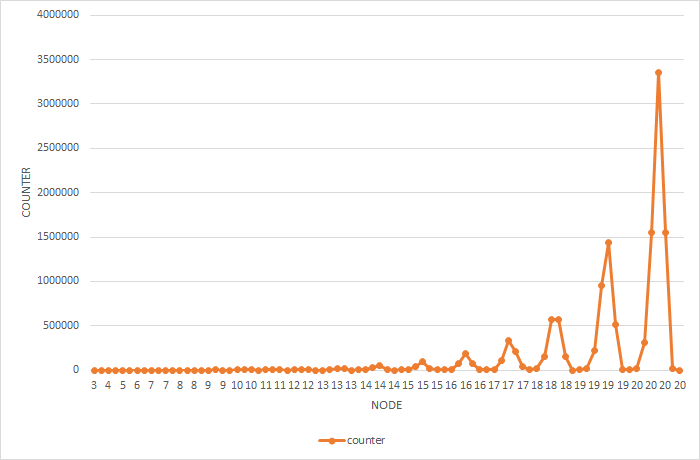
\includegraphics[width=1\linewidth]{imgs/exhaustiveCounterNodes20.png}
				\caption{Exhaustive - Counter vs Nodes vs $k$}
				\label{figure:exhaustiveCounterNodes20}
			\end{figure}
		
			\begin{figure}[!h]
				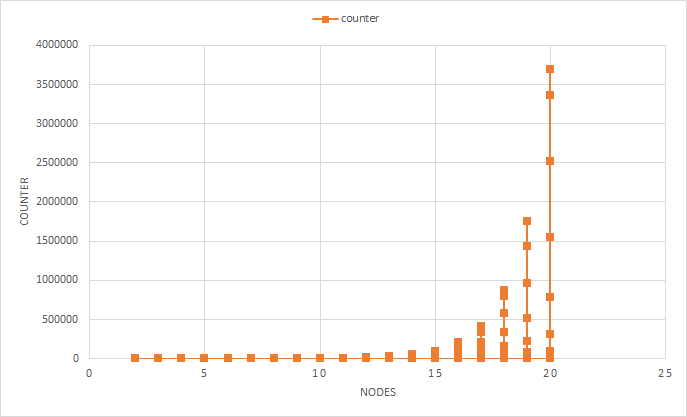
\includegraphics[width=1\linewidth]{imgs/exhaustiveCounterNodesSummary.png}
				\caption{Exhaustive (summary) - Counter vs Node vs $k$}
				\label{figure:exhaustiveCounterNodesSummary}
			\end{figure}
		
			\begin{figure}[!h]
				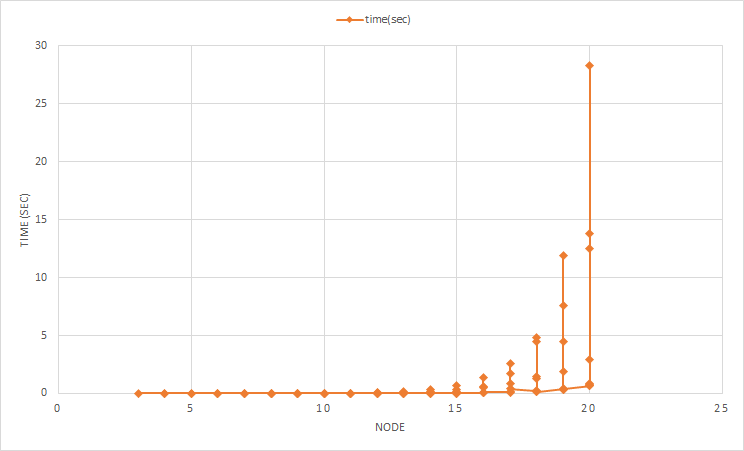
\includegraphics[width=1\linewidth]{imgs/exhaustiveTimeNodes20.png}
				\caption{Exhaustive - Time vs Node vs $k$}
				\label{figure:exhaustiveTimeNodes20}
			\end{figure}
		
			\begin{table}[!h]
				{\renewcommand{\arraystretch}{1.2}
				\begin{tabular}{|c|c|c|c|c|}
					\hline
					node&$k$&counter&ratio&time (secs)\\
					\hline
					3	&2&	9&	-&	0\\
					\hline
					4	&2	&24	&1.5	&0\\
					4	&3&	16	&0.67	&0.001\\
					\hline
					5&	2	&50	&2	&0\\
					5	&3	&50	&1	&0\\
					\hline
					6	&2	&90	&2.5	&0.001\\
					6	&3	&120	&1.333&	0\\
					6&	5	&36	&0.3	&0.001\\
					\hline
					10&	2&	450	&4.5&	0.003\\
					10&	3&	1200&2.67&	0.007\\
					10&	5&	2520&2.1&	0.0155\\
					10&	7&	1200&0.476&	0.0078\\
					\hline
					20&	2&	3800&	9.5&	0.674\\
					20&	3&	22800&	6	&0.791\\
					20&	5&	310080&	13.6&	2.82\\
					20&	7&	1550400&	5&	12.118\\
					20&	11&	3359200&	2.167&	27.414\\
					20&	13&	1550400	&0.462&	13.308\\
					20&	17&	22800	&0.0147&	0.817\\
					20&	19&	400&	0.0175&	0.632\\
					\hline
				\end{tabular}
				}
				\caption{Exhaustive - Output Snapshot}
				\label{table:exhaustiveOutputSnapshot}
			\end{table}
		
		\newpage
		\subsection{Greedy Heuristic}
			For each prime number $k$, for a given vertex, \textbf{Table \ref{table:greedyOutputSnapshot}} we presents a record of the number of operations (counter), the ratio of the number of operations (ratio) and the time (secs) the algorithm takes to complete execution. This is a snapshot of the output for the Greedy implementation is presented. A detailed result is given in the register output. \\
			
			Unlike in the case of the Exhaustive-Search, the time taken for the Greedy-search implementation is insignificant. The maximum time taken spent on the largest graph with twenty (20) nodes is barely three (3) milliseconds. The results output also show very good estimations by the greedy heuristics. An instance of this is described in the next section where out of three (3) locations, the greedy heuristics was able to correctly estimate two (2) of the locations. Out of two (2), it was able to correctly estimate one (1) of the locations.\\
			
			The time taken for larger graphs to complete looks more to be linear linear as seen in \textbf{Fig. \ref{figure:greedyTimeNodes20}}.
			
			\begin{figure}[!h]
				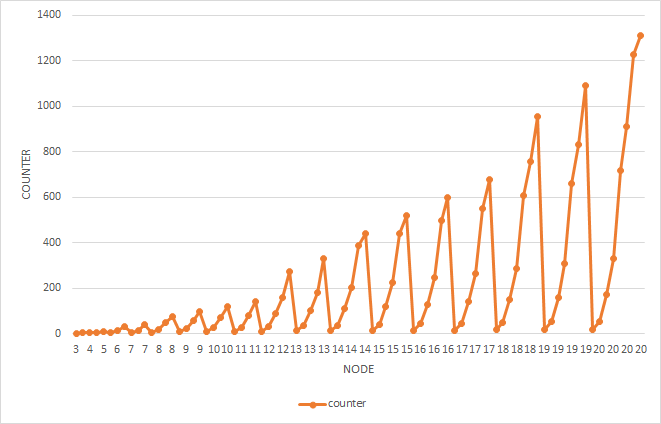
\includegraphics[width=1\linewidth]{imgs/greedyCounterNodes20.png}
				\caption{Greedy - Counter vs Nodes vs $k$}
				\label{figure:greedyCounterNodes20}
			\end{figure}
		
			\begin{figure}[!h]
				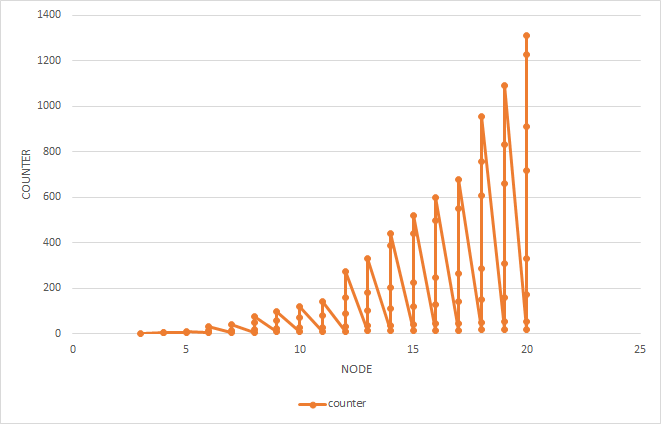
\includegraphics[width=1\linewidth]{imgs/greedyCounterNodesSummary.png}
				\caption{Greedy (summary) - Counter vs Node vs $k$}
				\label{figure:greedyCounterNodesSummary}
			\end{figure}
			
			\begin{figure}[!h]
				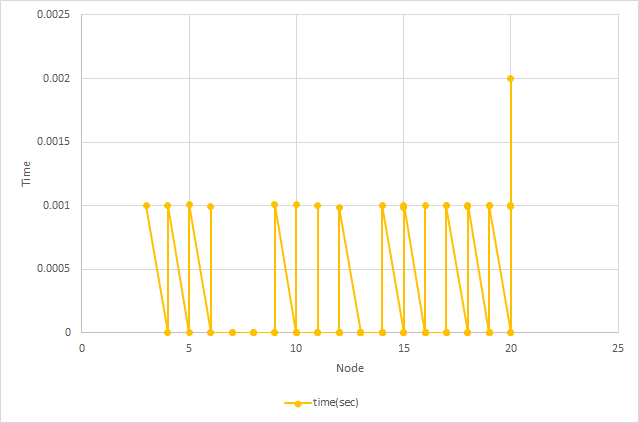
\includegraphics[width=1\linewidth]{imgs/greedyTimeNodes20.png}
				\caption{Greedy - Time vs Node vs $k$}
				\label{figure:greedyTimeNodes20}
			\end{figure}
			
			\begin{table}[!h]
				{\renewcommand{\arraystretch}{1.2}
					\begin{tabular}{|c|c|c|c|c|}
						\hline
						node&$k$&counter&ratio&time (secs)\\
						\hline
						3	&2	&3	&-	&0.0\\
						\hline
						4	&2	&2	&1	&0\\
						4	&3	&3	&1.5	&0.0\\
						\hline
						5	&2	&2	&0.667	&0\\
						5	&3	&3	&1.5	&0.001\\
						\hline
						6	&2	&2	&0.667	&0\\
						6	&3	&3	&1.5	&0\\
						6	&5	&5	&1.667	&0\\
						\hline
						10	&2	&2	&0.286	&0\\
						10	&3	&3	&1.5	&0.001\\
						10	&5	&5	&1.667	&0\\
						10	&7	&7	&1.4	&0.001\\
						\hline
						20	&2	&2	&0.118	&0\\
						20	&3	&3	&1.5	&0.001\\
						20	&5	&5	&1.667	&0.001\\
						20	&7	&7	&1.4	&0\\
						20	&11	&11	&1.571	&0.001\\
						20	&13	&13	&1.182	&0\\
						20	&17	&17	&1.308 &0.001\\
						20	&19	&19	&1.118	&0.001\\
						\hline
					\end{tabular}
				}
				\caption{Greedy - Output Snapshot}
				\label{table:greedyOutputSnapshot}
			\end{table}
		
		\newpage
		\subsection{Randomized Approach}
			A snapshot of result from the output register for this strategy is presented in \textbf{Table \ref{table:randomizedOutputSnapshot}} recording the number of operations, and time taken to complete each operation of $k$\\
			
			\textbf{Fig. \ref{figure:randomizedCounterNodes20}} shows a plot of the number of operations (counter) carried out for each $k$. As shown, we observe a linear relationship between the number of operations its corresponding graph node.\\
		
			The trend in time taken to complete an operation seems to be constant at about one (1) milliseconds as observed from \textbf{Fig. \ref{figure:randomizedTimeNodes20}}. This is the most fastest algorithm discussed so far. As a trade-off, there is no guarantee the obtained result is near optimal.
		
			\begin{figure}[!h]
				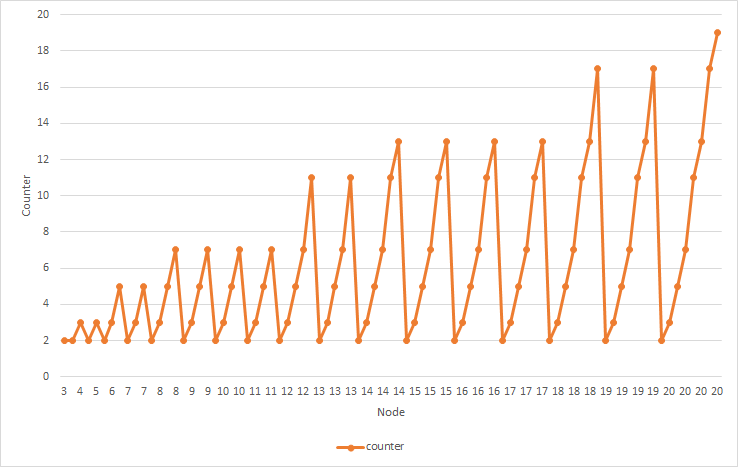
\includegraphics[width=1\linewidth]{imgs/randomizedCounterNodes20.png}
				\caption{Randomized - Counter vs Nodes vs $k$}
				\label{figure:randomizedCounterNodes20}
			\end{figure}
			
			\begin{figure}[!h]
				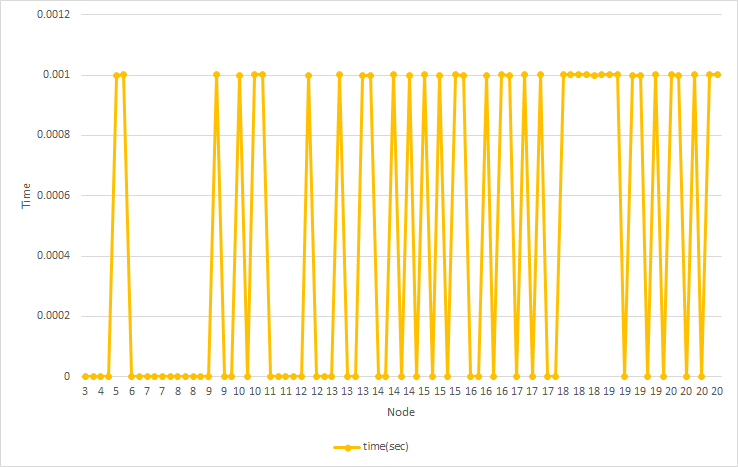
\includegraphics[width=1\linewidth]{imgs/randomizedTimeNodes20.png}
				\caption{Randomized - Time vs Node vs $k$}
				\label{figure:randomizedTimeNodes20}
			\end{figure}
			
			\begin{table}[!h]
				{\renewcommand{\arraystretch}{1.2}
					\begin{tabular}{|c|c|c|c|c|}
						\hline
						node&$k$&counter&ratio&time (secs)\\
						\hline
						3	&2	&3	&-	&0.001\\
						\hline
						4	&2	&4	&1.333	&0\\
						4	&3	&8	&2	&0.001\\
						\hline
						5	&2	&5	&0.625	&0\\
						5	&3	&11&	2.2&	0.001\\
						\hline
						6	&2	&6	&0.545	&0\\
						6	&3	&14	&2.333	&0.001\\
						6	&5	&31	&2.214	&0\\
						\hline
						10	&2	&10	&0.101	&0\\
						10	&3	&26	&2.6	&0\\
						10	&5	&71	&2.731	&0.0015\\
						10	&7	&120&	1.69	&0\\
						\hline
						20	&2	&20	&0.0184	&0\\
						20	&3	&56	&2.8	&0.001\\
						20	&5	&171	&3.054	&0\\
						20	&7	&330	&1.93	&0\\
						20	&11	&716	&2.17	&0.001\\
						20	&13	&911	&1.272	&0.001\\
						20	&17	&1225	&1.345 &0.002\\
						20	&19	&1312	&1.071	&0.001\\
						\hline
					\end{tabular}
				}
				\caption{Randomized - Output Snapshot}
				\label{table:randomizedOutputSnapshot}
			\end{table}
		
	\newpage
	\section{\label{outline:example-case} Example Case ($n=5$)}
		In this section, we consider instance problem of a graph with $|\mathcal{V}|=5$ vertices and $|\mathcal{E}|=10$ edges, as presented in \textbf{Fig. \ref{figure:n5}}. Hence, the $k$ values considered for this example are $[2,3]$ which are the expected prime numbers as described in the preamble. For this considered example, the Exhaustive-Search, Greedy and Random algorithms were implemented and their corresponding results analyzed.
		\begin{figure}[!h]
			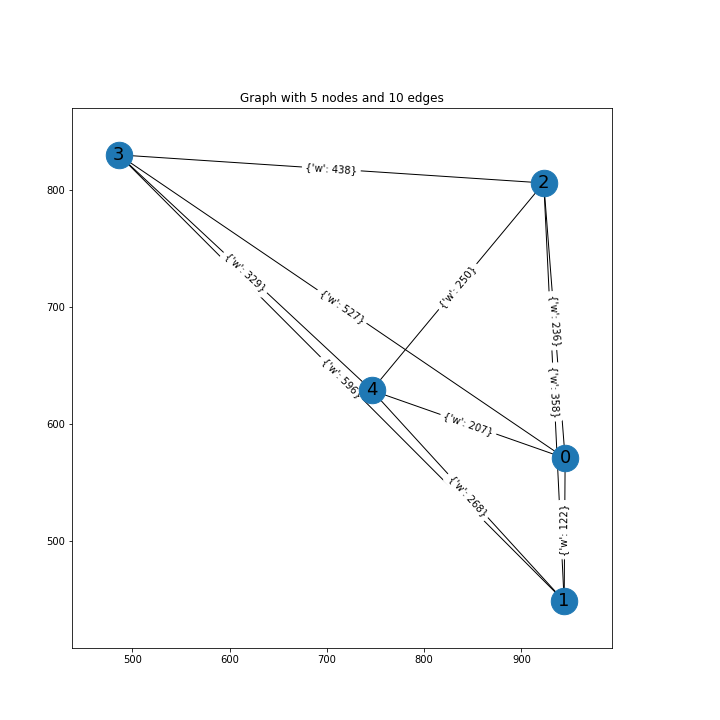
\includegraphics[width=\linewidth, height=0.8\linewidth]{imgs/n5.png}
			\caption{Graph With 5 vertices and 10 edges}
			\label{figure:n5}
		\end{figure}
	
		\textbf{Fig. \ref{figure:exhaustivek2_k3}} shows a graphical output of a solution to the above problem using the Exhaustive-Search, \textbf{Fig. \ref{figure:greedyk2_k3}} also represents a graphical optimal warehouse locations set using the Greedy Heuristics and \textbf{Fig. \ref{figure:randomizedk2_k3}} shows similar result/solution using a Randomized algorithm.\\
		
		The Exhaustive-Search implementation presents the optimal locations solution. As it can be observed, we have the Greedy heuristics able to provide a near optimal solution set. For \emph{k=2}, the Greedy implementation was able to correctly predict one (1) warehouse location and for \emph{k=3}, it correctly predicted two (3) warehouse locations. We can say these near-accurate estimation of the optimal solution set is as a result of the partial optimization implemented by the algorithm. If there is a coincidence of the Randomized algorithm correctly estimating a warehouse location, we can say the coincidence is due to chance and not based on some carefully chosen heuristics as can be seen for in the outputs.\\
		
		\begin{figure}[!h]
			\begin{tabular}{cc}
				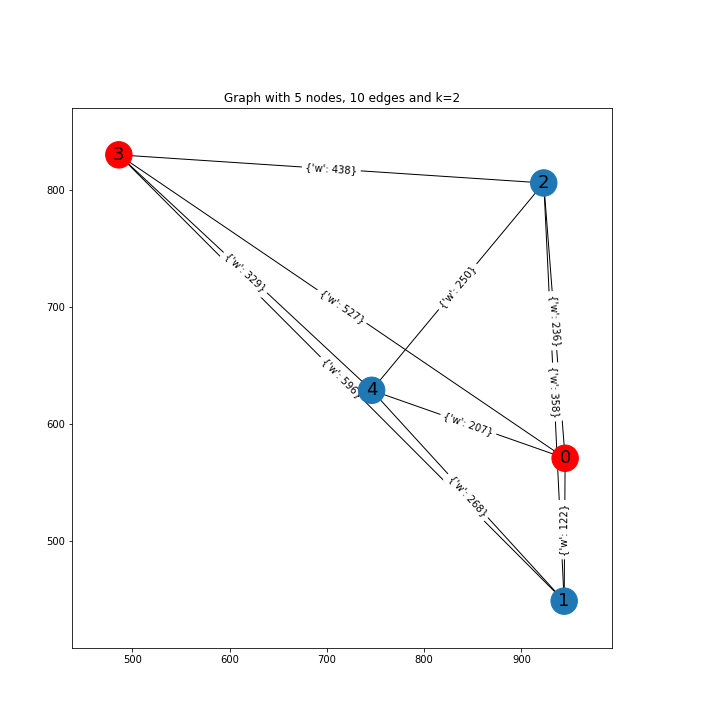
\includegraphics[width=0.5\linewidth]{imgs/exhaustive_n5_k2.png} &   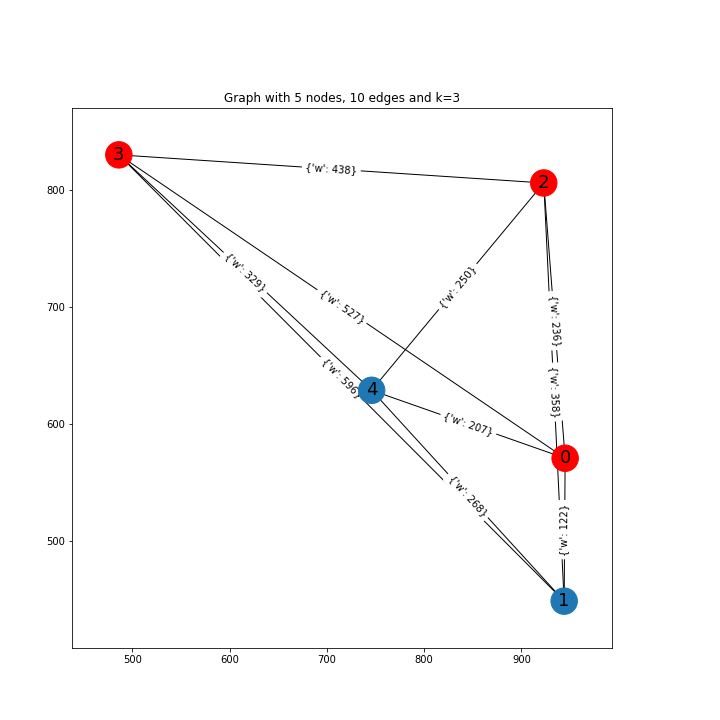
\includegraphics[width=0.5\linewidth]{imgs/exhaustive_n5_k3.png} \\
			\end{tabular}
			\caption{Exhaustive (k=2, k=3)}
			\label{figure:exhaustivek2_k3}
		\end{figure}
		
		\begin{figure}[!h]
			\begin{tabular}{cc}
				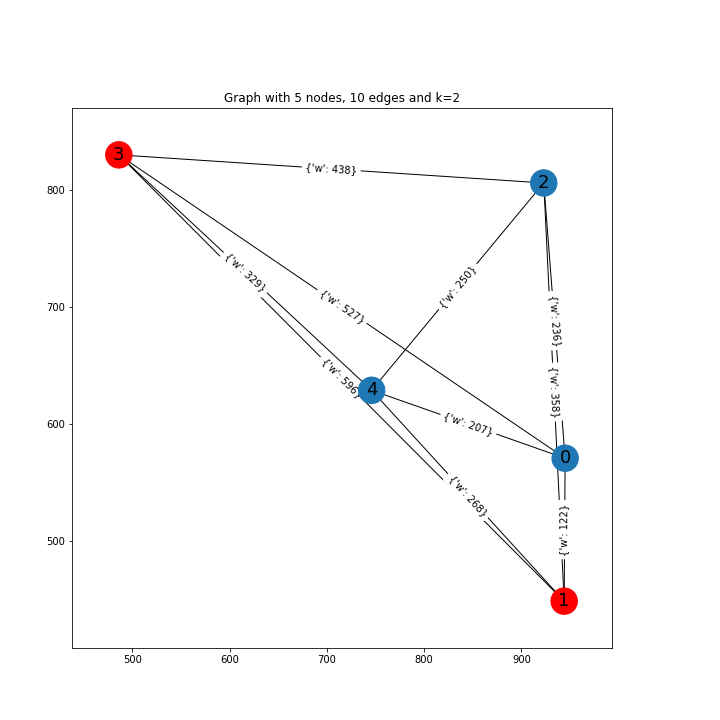
\includegraphics[width=0.5\linewidth]{imgs/greedy_n5_k2.png} &   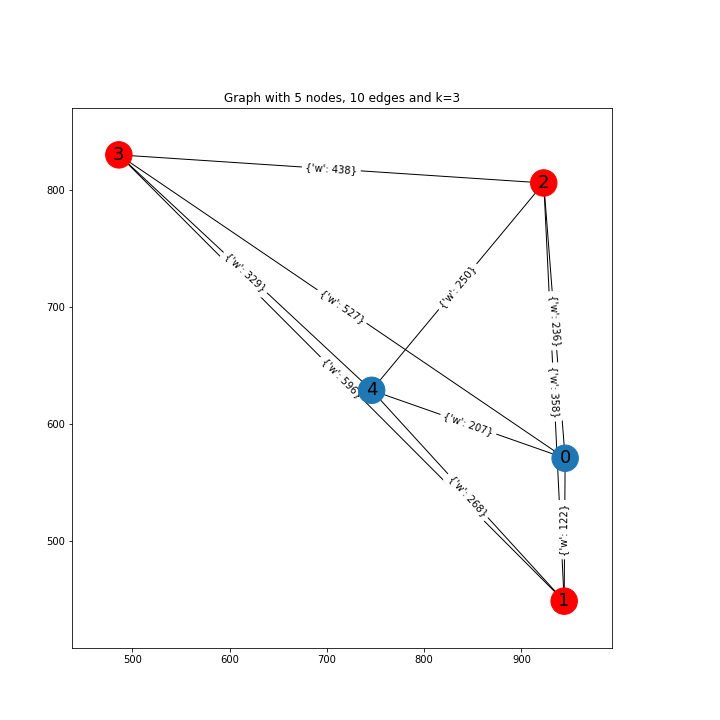
\includegraphics[width=0.5\linewidth]{imgs/greedy_n5_k3.png} \\
			\end{tabular}
			\caption{Greedy (k=2, k=3)}
			\label{figure:greedyk2_k3}
		\end{figure}
	
		\begin{figure}[!h]
			\begin{tabular}{cc}
				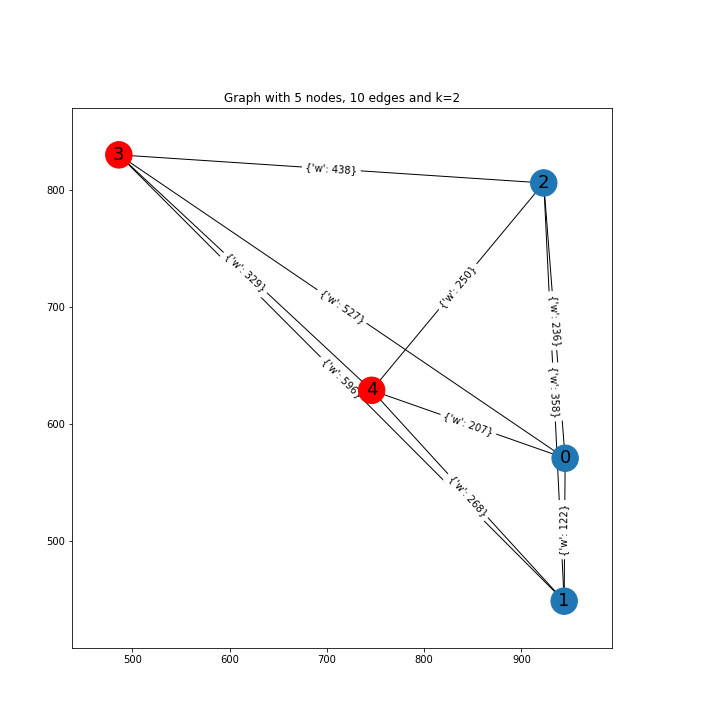
\includegraphics[width=0.5\linewidth]{imgs/randomized_n5_k2.png} &   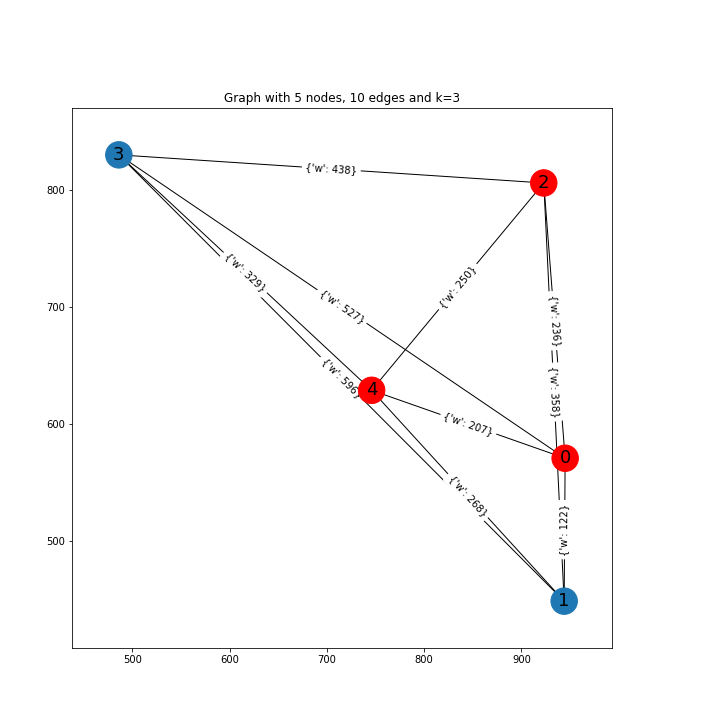
\includegraphics[width=0.5\linewidth]{imgs/randomized_n5_k3.png} \\
			\end{tabular}
			\caption{Randomized (k=2, k=3)}
			\label{figure:randomizedk2_k3}
		\end{figure}
	
	\newpage
	\section{\label{outline:conclusion} Conclusion}
		In conclusion we have seen that a Exhaustive-Search algorithm to solve the warehouse location problem is not feasible for large scale Graphs. The execution time is exponential. \\
		
		A Greedy Heuristic solution to this problem, is substantially more optimal running in what appears to be linear time for Graphs which would not even be thought possible to run compared to a brute force algorithm. This shows the importance of greedy heuristics, should an approximate solution to a problem be acceptable.\\
		
		With the Randomized algorithm, we observe a constant time for its execution regardless the size of its graph input. This is a very fast algorithm in obtaining an estimate which may be very far from optimal. The Greedy algorithm which is an extension of the naive randomized approach is our best shot which trades speed for accuracy.
	
	
	\bibliography{references} % use a field named url or \url{} for URLs
	% Note: the \bibliographystyle is set automatically
%	 \bibliographystyle{plain}
	
\end{document}
